%!TEX root = lab0.tex

\chapter*{Introduction}

Before diving into this computer networks lab course, it is useful to present some conventions first. \stress{Keep in mind that these conventions are introduced to make all of our lives easier.} In case of problems, it is easier to have a look at a lab setup if everyone sticks to the same rules.

\section{Practical Arrangements}
\subsection*{Group Practice}

The labs are performed in groups of two students. Within the next week, you need to form your groups. To register, subscribe to one of the groups that have been made available on Blackboard.

\subsection{Mininet Virtual Machine}

\subsubsection{Getting the VM}
We provide a Virtual Machine with an Ubuntu variant and IPMininet installed. You can download this image from \url{https://student.idlab.uantwerpen.be/computernetwerken/}. There are two distinct VMs available: one for running on Intel-based computers (``Computernetwerken-AMD64''), and one for running on Apple silicon (``Computernetwerken-ARM'').

If you are using a computer running on Intel architecture, we suggest you use Virtualbox (\url{https://www.virtualbox.org/}) for running your Virtual Machine. After installing Virtualbox, set up your machine as follows:
\begin{enumerate}
\item Download and open the Computernetwerken-AMD64.ova file.
\item You should now see the VirtualBox Import Appliance.
\item Click the Import button, and the Virtual Machine is imported in Virtualbox. This can take a few minutes.
\end{enumerate}

When you are using a machine running on Apple silicon, A VM is provided that has been made with the ``UTM'' virtualisation software. UTM is freely downloadable from the App Store. If your are using Apple silicon, set up your machine as follows after installing the UTM appliance:
\begin{enumerate}
	\item Download and open the Computernetwerken-ARM.utm.zip file.
	\item Unpack the zip file.
	\item You should now see the UTM Appliance.
	\item Double-click the Computernetwerken-ARM.utm file to import it into UTM.
	\end{enumerate}

Now you should be able to start your virtual machine. The password is \incommand{mvkbj1n}. Open a terminal and type \incommand{sudo mn} to verify if the machine is indeed installed correctly. If everything is fine, you should see Mininet starting up and creating a basic network.

\subsubsection{Sudo}
When working in the terminal either use \incommand{sudo} before each command to get root privileges.
\begin{cmdblock}[gobble=1]
	% sudo ip addr add 2001:db8::1/64 dev eth0
\end{cmdblock}

Or type in \incommand{sudo su -} at the beginning of each new terminal session to keep working with root privileges.

You will be asked for a password when using the \incommand{sudo} command, the default password on the VM is \incommand{mvkbj1n}.

\section{\acs{ipv6} Address Notation}
Throughout the course, \ac{ipv6} addresses are used. The following conventions always apply:
\begin{itemize}
\item For \stress{documentation purposes}, \ac{ipv6} addresses are used that belong to the \emph{documentation range}, i.e., \texttt{2001:db8::/32}. These addresses are \stress{never} used on actual interfaces!
\item The actual \ac{ipv6} addresses that are configured on the PCs and routers, will always belong to the \emph{unique local unicast} range, which is defined as \texttt{fc00::/8} and \texttt{fd00::/8}.
\end{itemize}


\section{Communication}

Do not hesitate to seek help! The objective of this course is to get a hands on experience in networking, not in debugging devices or software. If you get stuck, try to find a solution using one of the following channels:

\begin{itemize}
	\item Send an e-mail: \href{mailto:johan.bergs@uantwerpen.be}{johan.bergs@uantwerpen.be}, or \href{mailto:andrei.belogaev@uantwerpen.be}{andrei.belogaev@uantwerpen.be}
\end{itemize}

All information about this course will be posted on Blackboard. Blackboard will also be used to collect your reports.

\section{Course Evaluation}
\addcontentsline{toc}{chapter}{Course Evaluation}

This course will be evaluated based on the lab reports that you will need to complete and send in before the given deadlines.

\subsection*{Evaluation Criteria and Deadlines}
\subsubsection{Evaluation Criteria (for groups of two)}
\begin{enumerate}
\item Each group member receives the same grade.
\item The final grade is calculated as an average of the grades of the individual lab reports.
\item The lab reports are subject to deadlines. If a lab report is not handed in by 23:59 on the day of the deadline, the grade for that lab report will automatically be 0/20. Consult Blackboard for this year's deadlines.
\end{enumerate}

\section{Lab Reports}
\addcontentsline{toc}{chapter}{Lab Reports}

\subsection*{Writing Lab Reports}
This course expects you to write your lab report using \LaTeX. To make things easier, you will be provided with a template for each lab which already contains the questions you need to fill in. The idea is that you answer the questions in separate files in the \path{solutions/} folder. You are supposed to send in a compiled PDF file, the \path{.tex} solution files and your traces.

Download the lab report templates from Blackboard. They will all be bundled in one file \path{Lab.tar.gz}. Unpack this file and you will see the following structure:

\dirtree{%
	.1 /.
	.2 Lab0/.
	.2 Lab1/.
		.3 graphics/ \DTcomment{Graphical resources used in lab.}.
		.3 solutions/ \DTcomment{Contains all your solutions.}.
			.4 L1-1-1.tex \DTcomment{Answer to first question of the lab.}.
		.3 traces/ \DTcomment{Place your traces here. Mostly pcap, txt and pdf files.}.
		.3 lab1.tex \DTcomment{Compile this file to create lab1.pdf.}.
		.3 main1.tex \DTcomment{Body of lab1. Don't edit directly.}.
	.2 Lab2/ \DTcomment{Same as Lab1/.}.
	.2 Lab3/.
	.2 \ldots .
	.2 acro.text \DTcomment{List of acronyms.}.
	.2 bibliography.bib \DTcomment{Bibliography.}.
	.2 footer.tex \DTcomment{Don't edit this file.}.
	.2 groupid.tex \DTcomment{Add your name and group id in this file.}.
	.2 header.tex \DTcomment{Don't edit this file.}.
	.2 labo.tex \DTcomment{Concatenation of all labs.}.
}
Each of the labs needs to be submitted separately, so make sure you do not use any files outside of the directory of the lab.

\subsubsection{Using \LaTeX~on your own computer}
Try to compile the \path{lab0.tex} file with:
\begin{cmdblock}[gobble=1]
	pdflatex lab0.tex
\end{cmdblock}
This should work and create the file \path{lab0.pdf}.

\remark You might get an error message in the following labs that looks like this :
\begin{verbatim}
! You can't use `macro parameter character #' in vertical mode.
#
Add your group information to groupid.tex and remove this line.
\end{verbatim}
This tells you that you need to add your name and group id to the file \path{groupid.tex}. After you updated the information, remove the line starting with '\#' and the lab should compile without errors.

\subsubsection{Using Overleaf.com to write \LaTeX}
You can also upload all your source files to \url{Overleaf.com}, this is an online tool that allows you to write \LaTeX and generate pdf files. Create a new project for every lab, and upload all files to this project (make sure you keep the directories as they are). You can share an overleaf project with the student you are working with.

In Menu, you can choose to download the source code and the generated the pdf, both should be uploaded to Blackboard.

\subsubsection{Answering questions}

You can then begin to answer the questions in the lab. These will look like this:

\begin{exercise}{}
	\question{What is the answer to life the universe and everything?}{1}


Notice that the blue box with the question number is clickable. When you click the question, your default text editor should open and display the file \path{solutions/L0-1-1.tex} (not in Overleaf.com).

\remark Depending on the program you use to view PDF documents, you might need to change some security settings to get this to work. For example on Linux you can disable apparmor for evince (default PDF viewer) with the following commands:
\begin{cmdblock}
	sudo ln -s /etc/apparmor.d/usr.bin.evince /etc/apparmor.d/disable/usr.bin.evince
	sudo /etc/init.d/apparmor restart 
\end{cmdblock}

\remark This disables all security limitations imposed by apparmor on evince. Use these commands at your own risk.

Sometimes you will be asked to include data, or write a python script that specifies the topology for the following exercise. You should save all files in the \path{traces/} directory with the name given in the exercise. If you do this correctly, you can then use the \verb|\includetrace{}| command to include the data from a file in the traces directory.

For example: if you want to include the file \path{traces/L0-1-2.txt} in question 2 of exercise 1 in lab 0, all you need to type is \verb|\includetrace{txt}| . The prefix ``\path{traces/L0-1-2.}'' is automatically added. Give it a try: edit \file[2]{txt} so that it contains some text, and include it.

\question{Include \file[2]{txt} below.}{1}

Of course not all traces need to be included in the lab. Often you will be asked to refer to traces or link them. Sometimes this has even been done for you. In this case you should use the \verb|\linktrace{}| command. This allows you to link to trace files much like questions link to their answers. The linktrace command is a little bit smarter than includetrace. It will only link to trace files when they are present. If this is the case, the link will be blue and you should be able to click it. If not, the text is red and not clickable. Here is an example:

\question{Refer to \file[3]{pcap} and \file[3]{txt}.}{1}
As you can see, the file \file[3]{txt} is present, but \file[3]{pcap} is not.

When you encounter a \LaTeX error that you cannot work around, use the verbatim environment.

\verb!\begin{verbatim}!

\verb!\end{verbatim}!

\end{exercise}

\subsection*{Installing \LaTeX}

Having issues installing \LaTeX on your own laptop? Check \url{http://www.latex-project.org/get/}.

\subsection*{Answering Questions}
When answering a question in your lab report, keep the following in mind:
\begin{itemize}
	\item Read the question carefully. If you are asked to compare two things, then do so. Do not describe one and forget about the other. Comparing also means that you do not describe both items separately, but that you describe the similarities and differences between them.
	\item Most answers can be short, but make sure you include all necessary information.
	\item Only answer the question, otherwise you may lose points even when you include the correct answer. If you are asked to give a \ac{mac} address, for example, only give the \ac{mac} address and do not give the \ac{ipv6} address as well.
	\item If you are asked to give examples by giving packet IDs from specific packets in a trace file, then do so. Take extra care that you are referring to the correct trace file, especially if you made several traces for the same exercise.
	\item Give scientific answers. For example, you should write ``The ping in this setup is five times faster than in the previous setup''. Do not write ``There is a huge speed difference.'' or ``In this scenario, the ping is way faster.''
\end{itemize}

\newpage
\section{Lab 0: Introduction}\label{sec:lab0}
In this first lab, you will acquaint yourself with the tools we are going to use this semester.

\subsection{Basics of Wireshark}
Wireshark is a network protocol analyser with a graphical user interface. Using Wireshark, you can interactively capture and examine network traffic, view summaries and get detailed information for each packet. Wireshark can be downloaded from \url{https://www.wireshark.org}.

\begin{exercise}{Running Wireshark}
This exercise walks you through the steps of capturing and saving network traffic with Wireshark. The exercise is conducted on your own computer.

\begin{figure}[ht]
	\centering
	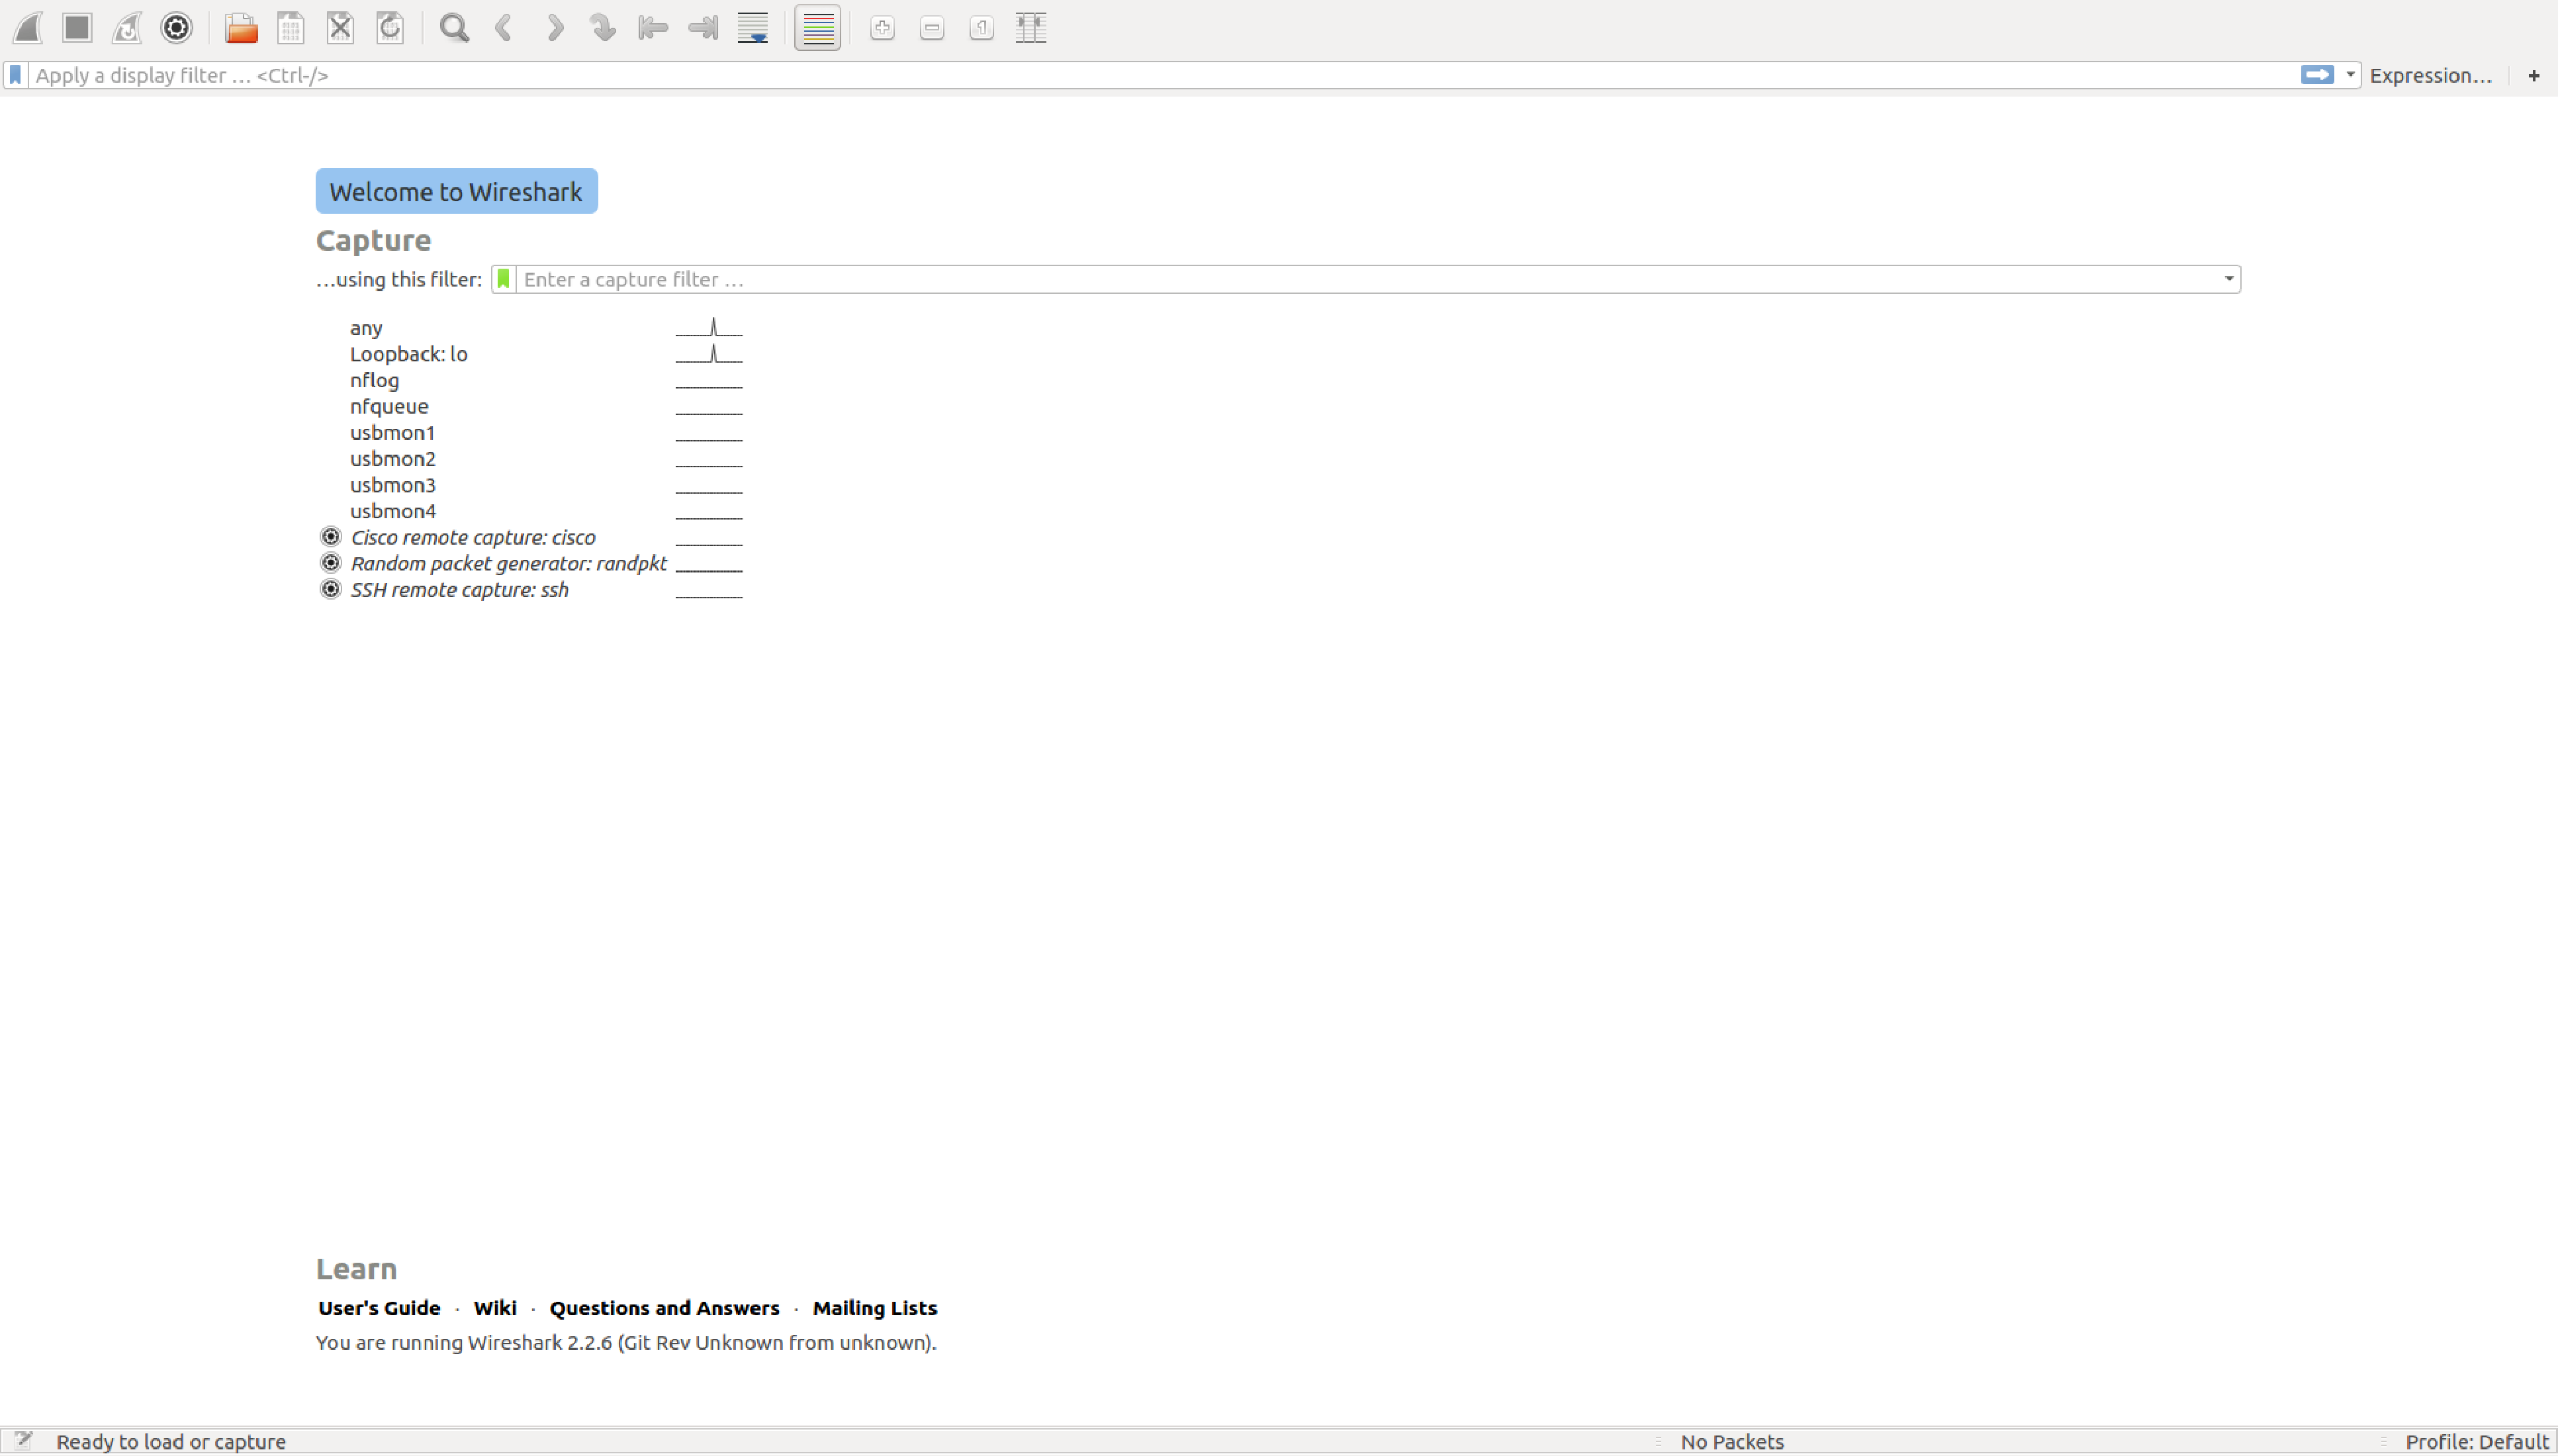
\includegraphics[width=\linewidth]{graphics/wireshark-main}	
	\caption{Wireshark Main Window.}
	\label{fig:lab1-wireshark-main}
\end{figure}

\begin{enumerate}
	\item Starting Wireshark: You can start Wireshark from a terminal with the command \incommand{wireshark} or from the desktop.
	
	This displays the Wireshark main window on your desktop as shown in figure \ref{fig:lab1-wireshark-main}.
	\item Selecting the capture options: use the instructions in figure \ref{fig:lab1-capture-options} to set the options of Wireshark in preparation for capturing traffic. Use the same options in other labs, whenever Wireshark is started.
		\par
		\begin{minipage}{\linewidth}
			\begin{framed}
				\centering
				\textbf{Selecting capture preferences in Wireshark}
				\begin{enumerate}
					\item From the main window, select ``Capture:Options''.
					\item This displays the following ``Capture Preferences'' window:\par
						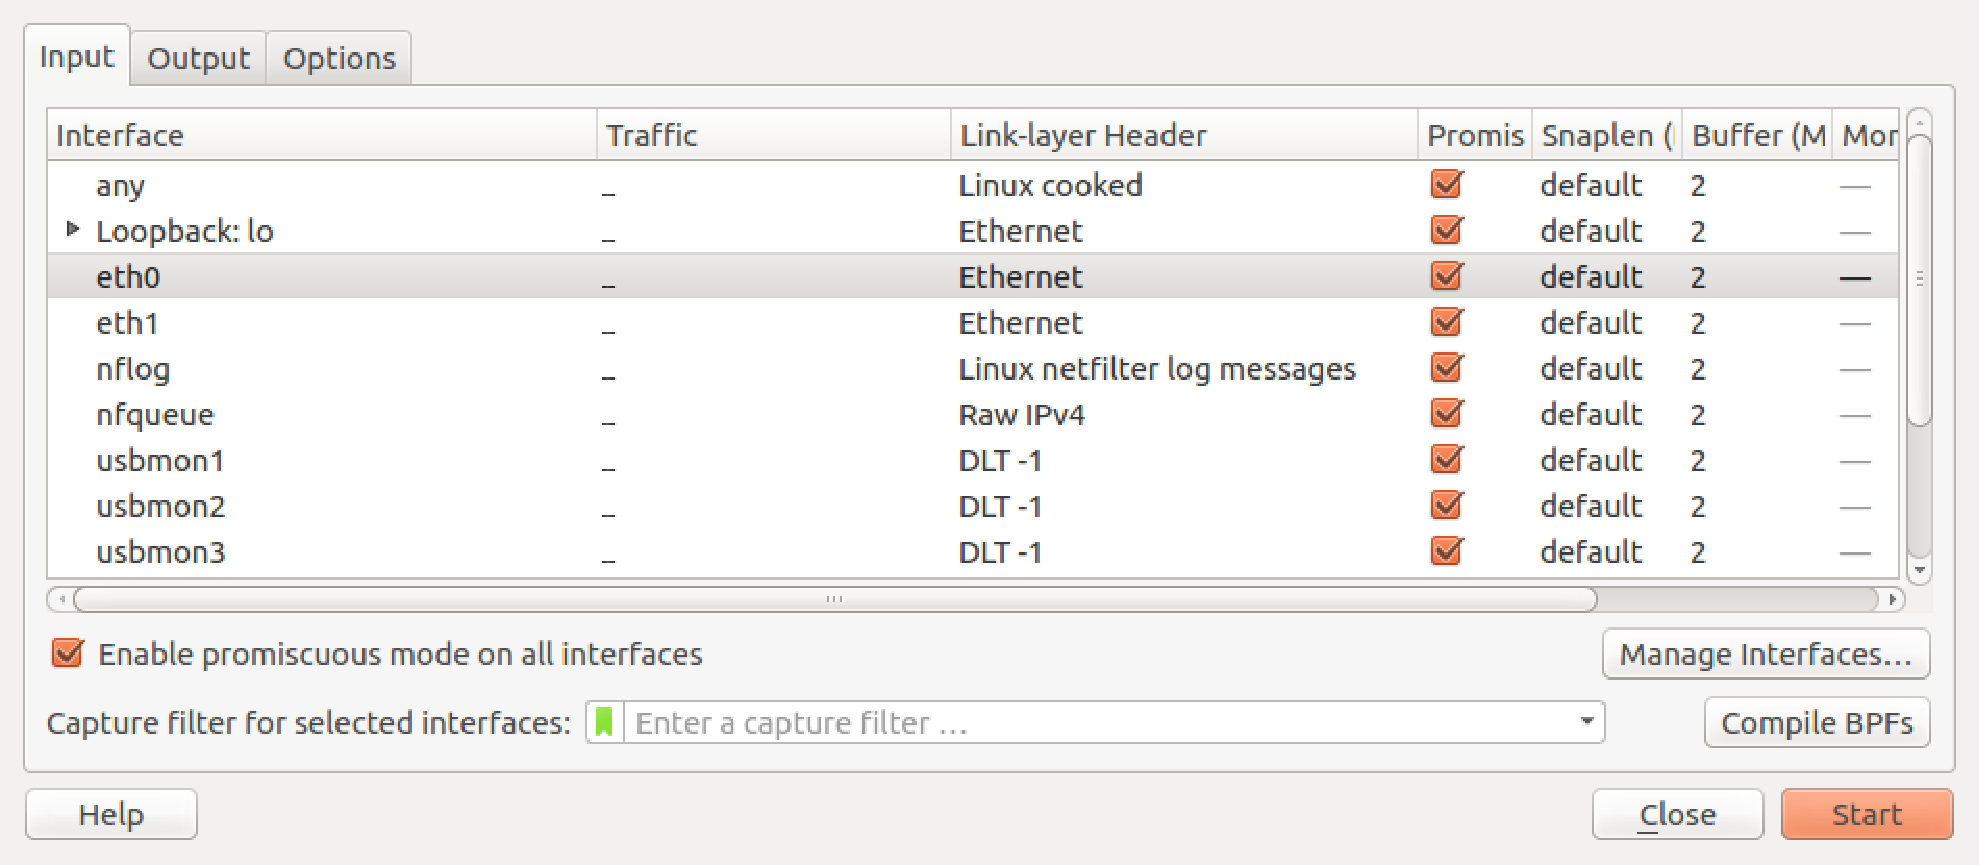
\includegraphics[width=0.85\linewidth]{graphics/wireshark-capture-options-1}
						\par
						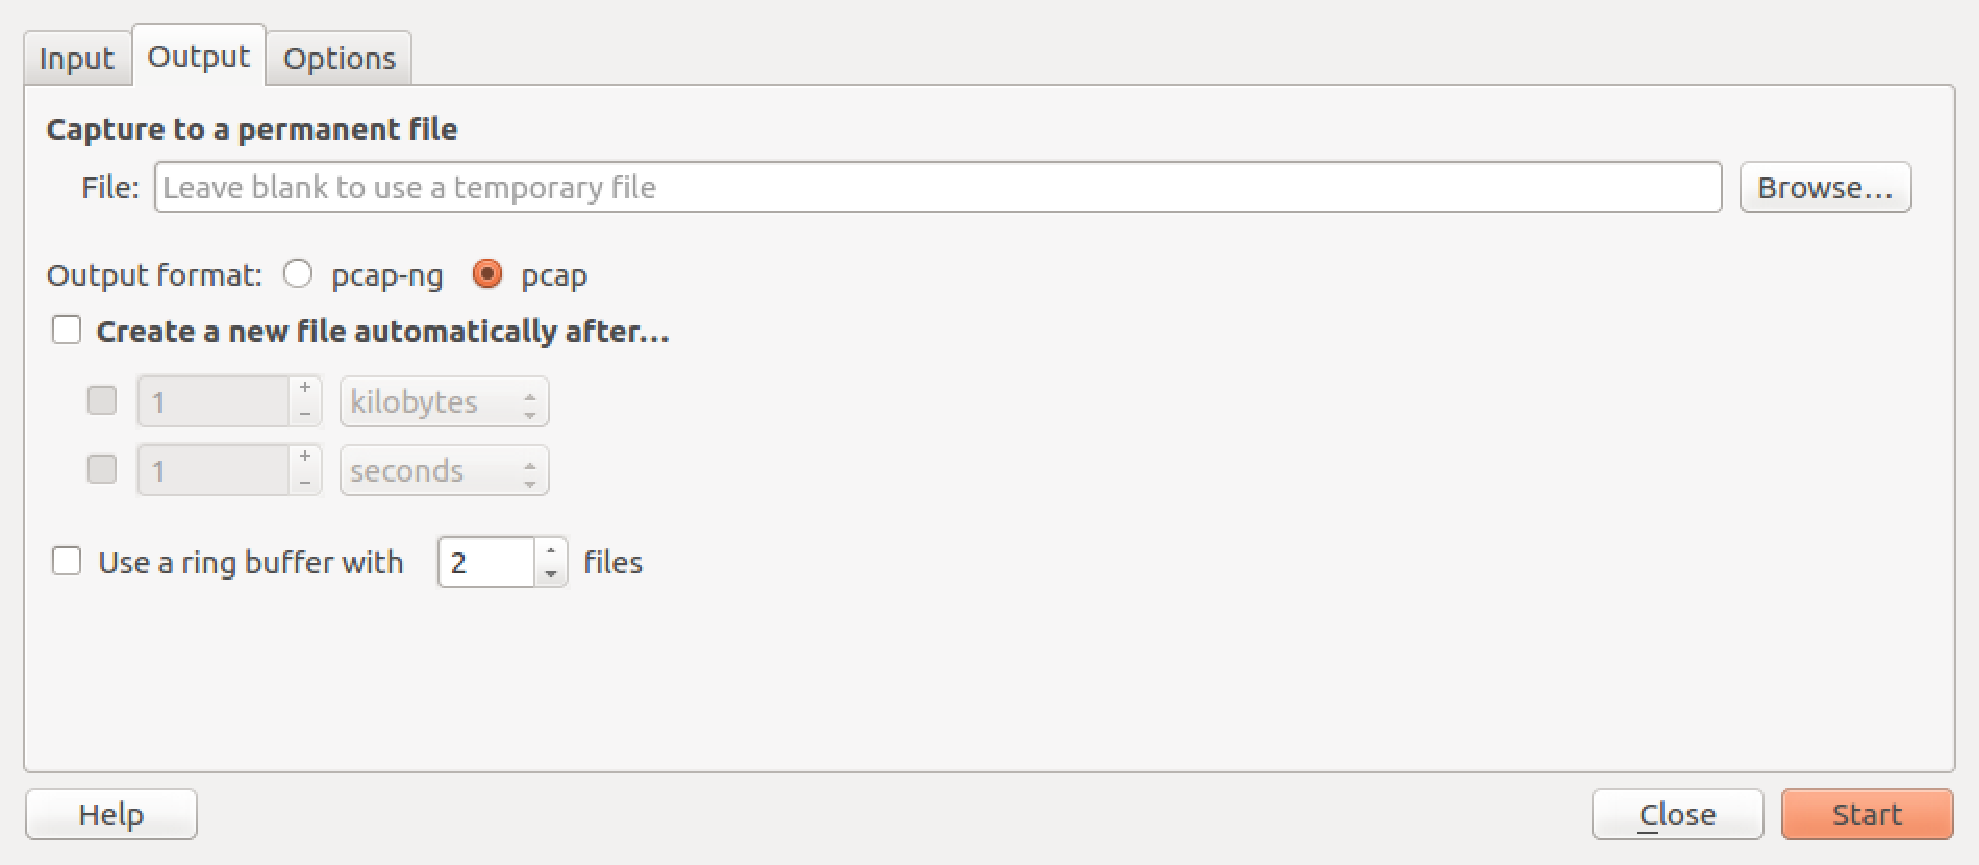
\includegraphics[width=0.85\linewidth]{graphics/wireshark-capture-options-2}
						\par
						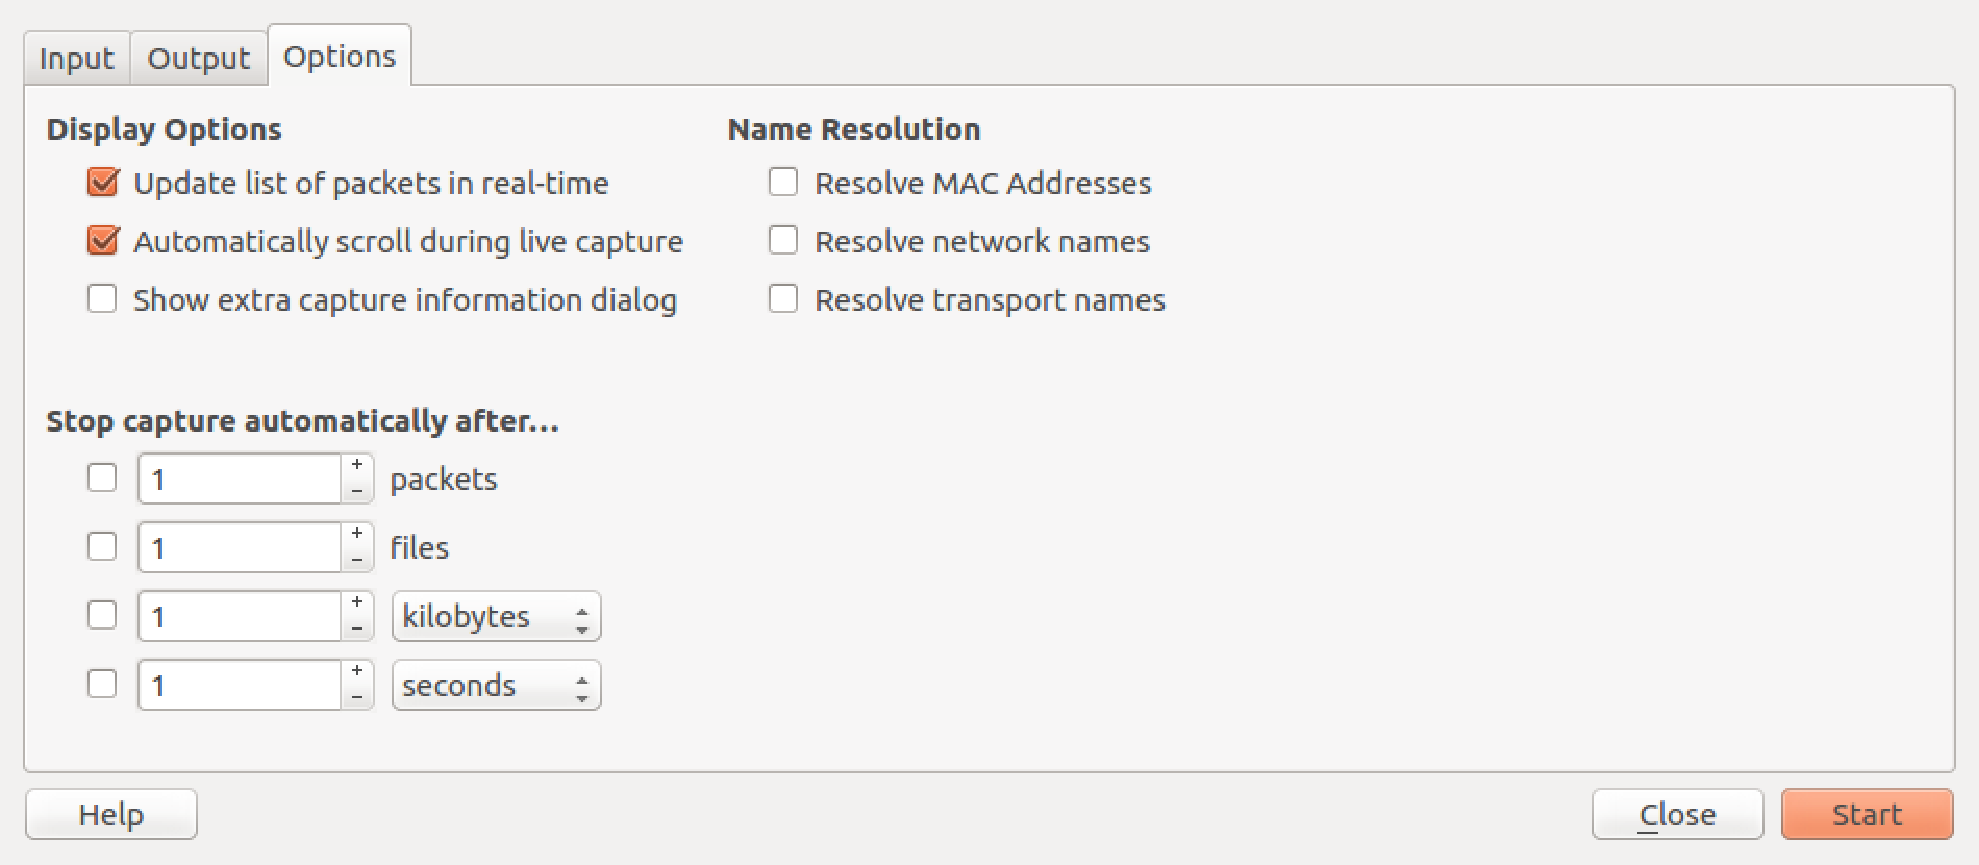
\includegraphics[width=0.85\linewidth]{graphics/wireshark-capture-options-3}
						\begin{itemize}
							\item Select \incommand{eth0} in ``Interface''.
							\item Select ``Use promiscuous mode on all interfaces''.
							\item Select ``Update list of packets in real time''.
							\item Select ``Automatically scroll during live capture''.
							\item Unselect ``Resolve MAC addresses''.
							\item Unselect ``Resolve network-layer names''.
							\item Unselect ``Resolve transport-layer name''.
						\end{itemize}
				\end{enumerate}
			\end{framed}
			\captionof{figure}{General capture settings for Wireshark}
			\label{fig:lab1-capture-options}
		\end{minipage}

	\item Starting the traffic capture: Start the packet capture by clicking ``Start'' in the ``Capture Options'' window.

	\item Generating traffic: in a separate window, execute a ping to \url{www.google.be}. Limit the amount of pings to 5. This is done by executing the following command:
	\begin{cmdblock}[gobble=2]
		% ping -c 5 www.google.be
	\end{cmdblock}
	
	Observe the output in Wireshark's main window. Click and highlight a captured packet in the Wireshark window, and view the headers of the captured traffic.

	\item Stopping the traffic capture: click ``Stop'' in the window ``Ethernet Capture''.
	\item Saving captured traffic: save the results of the captured traffic as libpcap file called \file{pcap}. 
			
			\remark If you select ``Save'' in the ``File'' menu, the captured data is saved in the format of a libpcap file. This format can be interpreted by both tcpdump and Wireshark. Measurements saved in libpcap format can be analysed at a later time.
			
			\remark \textbf{Always include binary libpcap traces with your report. Without the trace files, it is impossible to verify the validity of your answers. Keep in mind that, when answering questions that refer to a trace file, you will get no points if the trace file is not included, even if the answer is the correct one!}
\end{enumerate}

\question{Using the captured ping packets, describe which fields are present in the \ac{icmp} header. What is the amount of data present in the packet? How much bytes are required (in total) to actually transmit this data?}{2}

\end{exercise}

\newpage
\subsection{Creating virtual networks with IPMininet}
To be able to perform exercises on various network topologies, we use virtual networks created with IPMininet. This tool allows us to write a python script that describes the full topology, after which we can use this topology to run our tests. IPMininet is an extension of Mininet which allows to use both \ac{ipv4} and \ac{ipv6} addresses.

\begin{exercise}{Creating a Mininet topology}
When we want to create our own network topology, we define this network in a Python script which we can load into Mininet. This is done by using the API provided by Mininet. This script has the following structure and can be found in \path{solutions/mininet.py}:

\lstinputlisting{solutions/mininet.py}

We can now add hosts, switches and routers by using the following methods:
\begin{itemize}
	\item \texttt{self.addHost(hostname)}
	\item \texttt{self.addSwitch(switchname)}
	\item \texttt{self.addRouter(routername)}
\end{itemize}

This will create the hosts, switches and routers. The next step is to link them together to form the correct topology, we can do this using \texttt{self.addLink(node1, node2)}. For every link you define, a network interface is created on the connecting nodes. Now we can set the IP addresses (both IPv4 and IPv6) of these interfaces using the \texttt{addParams} method.

\begin{figure}[ht]
	\centering
	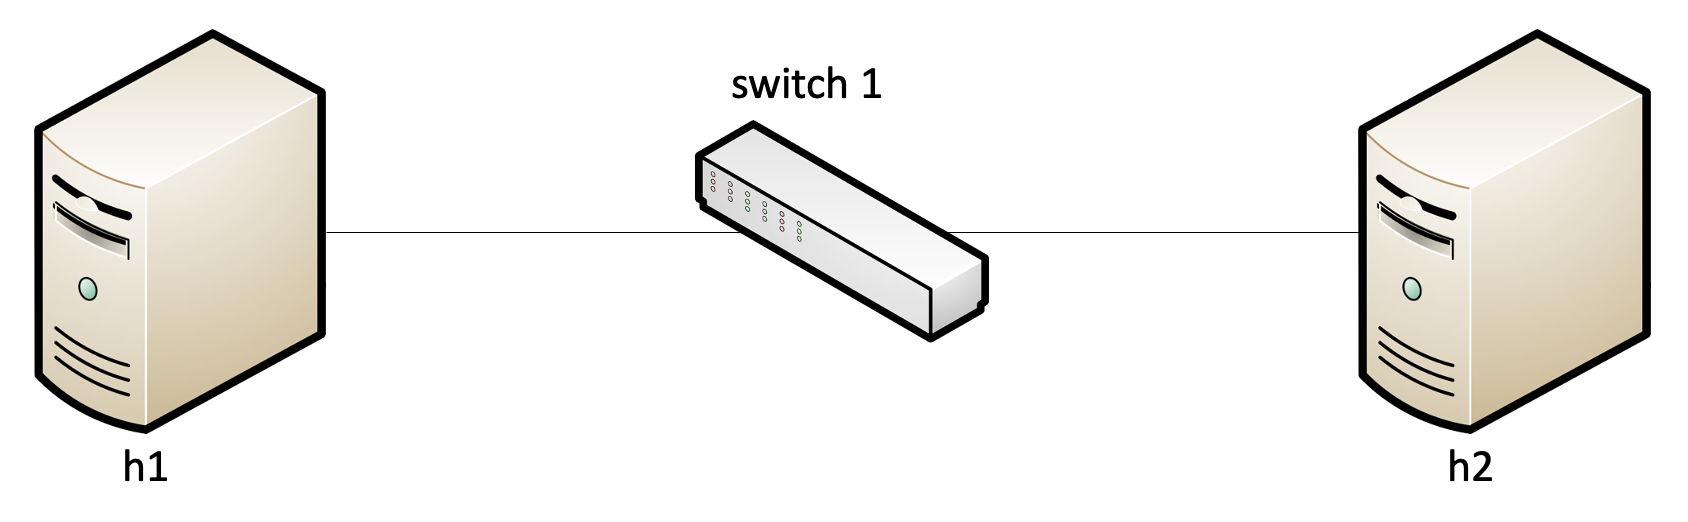
\includegraphics[width=0.8\linewidth]{graphics/Lab0-Mininet1.png}	
	\caption{Our first network topology, using 2 hosts and 1 switch}
	\label{fig:wireshark-http}
\end{figure}
\newpage

\begin{table}[ht]
	\centering
	\begin{tabular}{| c | c | c |}	
		\hline
		\textbf{Host} & \textbf{\ac{ipv6} address of eth0}  & \textbf{\ac{ipv4} address of eth0} \\ \hline
		h1 & \texttt{fc00:0:0:1::1/64} & \texttt{192.168.1.1/24} \\ 
		h2 & \texttt{fc00:0:0:1::2/64} & \texttt{192.168.1.2/24} \\
		\hline
	\end{tabular}
	\caption{\ac{ip} addresses for Exercise 3}
	\label{tab:mininet1}
\end{table}

To implement the topology we now have to add a few lines to the \path{mininet.py} script:

\lstinputlisting{solutions/L0-3-1.py}

To run this network we need to run our Python script. The script will start the Command Line Interface for mininet from which we can interact with the different hosts and components of the network.

Before you run your assignments on these networks, you first have to make sure that the configuration is correct. Mininet has some built in commands that makes it easier for you to check all connections between nodes. Try the following command:
\begin{cmdblock}[gobble=2]
	% pingall
\end{cmdblock}
You see that this command issues a ping command from all nodes to all nodes and displays which nodes are able to communicate which each other.

You can also run commands from one of the hosts, you do this by first entering the host name and then the command you want to perform on this host. If we want to use the ping command on host \textbf{h1} to check if we can reach host \textbf{h2}, you can use the following command:
\begin{cmdblock}[gobble=2]
	% h1 ping -c 3 h2
\end{cmdblock}
This command sends 3 ping requests to host \textbf{h2} and displays the response it receives. Instead of using the hostname we can also use the IP address of host \textbf{h2}:
\begin{cmdblock}[gobble=2]
	% h1 ping -c 3 192.168.1.2
\end{cmdblock}

You can also check the network interfaces of the different hosts by using \incommand{ifconfig}. Use this command to get an overview of the settings of the network interfaces of host \textbf{h2}. Copy the generated output to \file{txt}.
\end{exercise}

\begin{exercise}{Creating a more complex Mininet topology}\label{ex:mininet_complex}
Look at the topology in Figure \ref{fig:mininet2} and write a Python script that runs this topology in Mininet. The IP addresses to use are listed in Table \ref{tab:lab1-ip-addresses}. Save the file as \file{py}. Use \incommand{pingall} to test if all hosts can reach each other. You can assign an IP address to the interface of a router like you do for hosts.

\begin{figure}[ht]
	\centering
	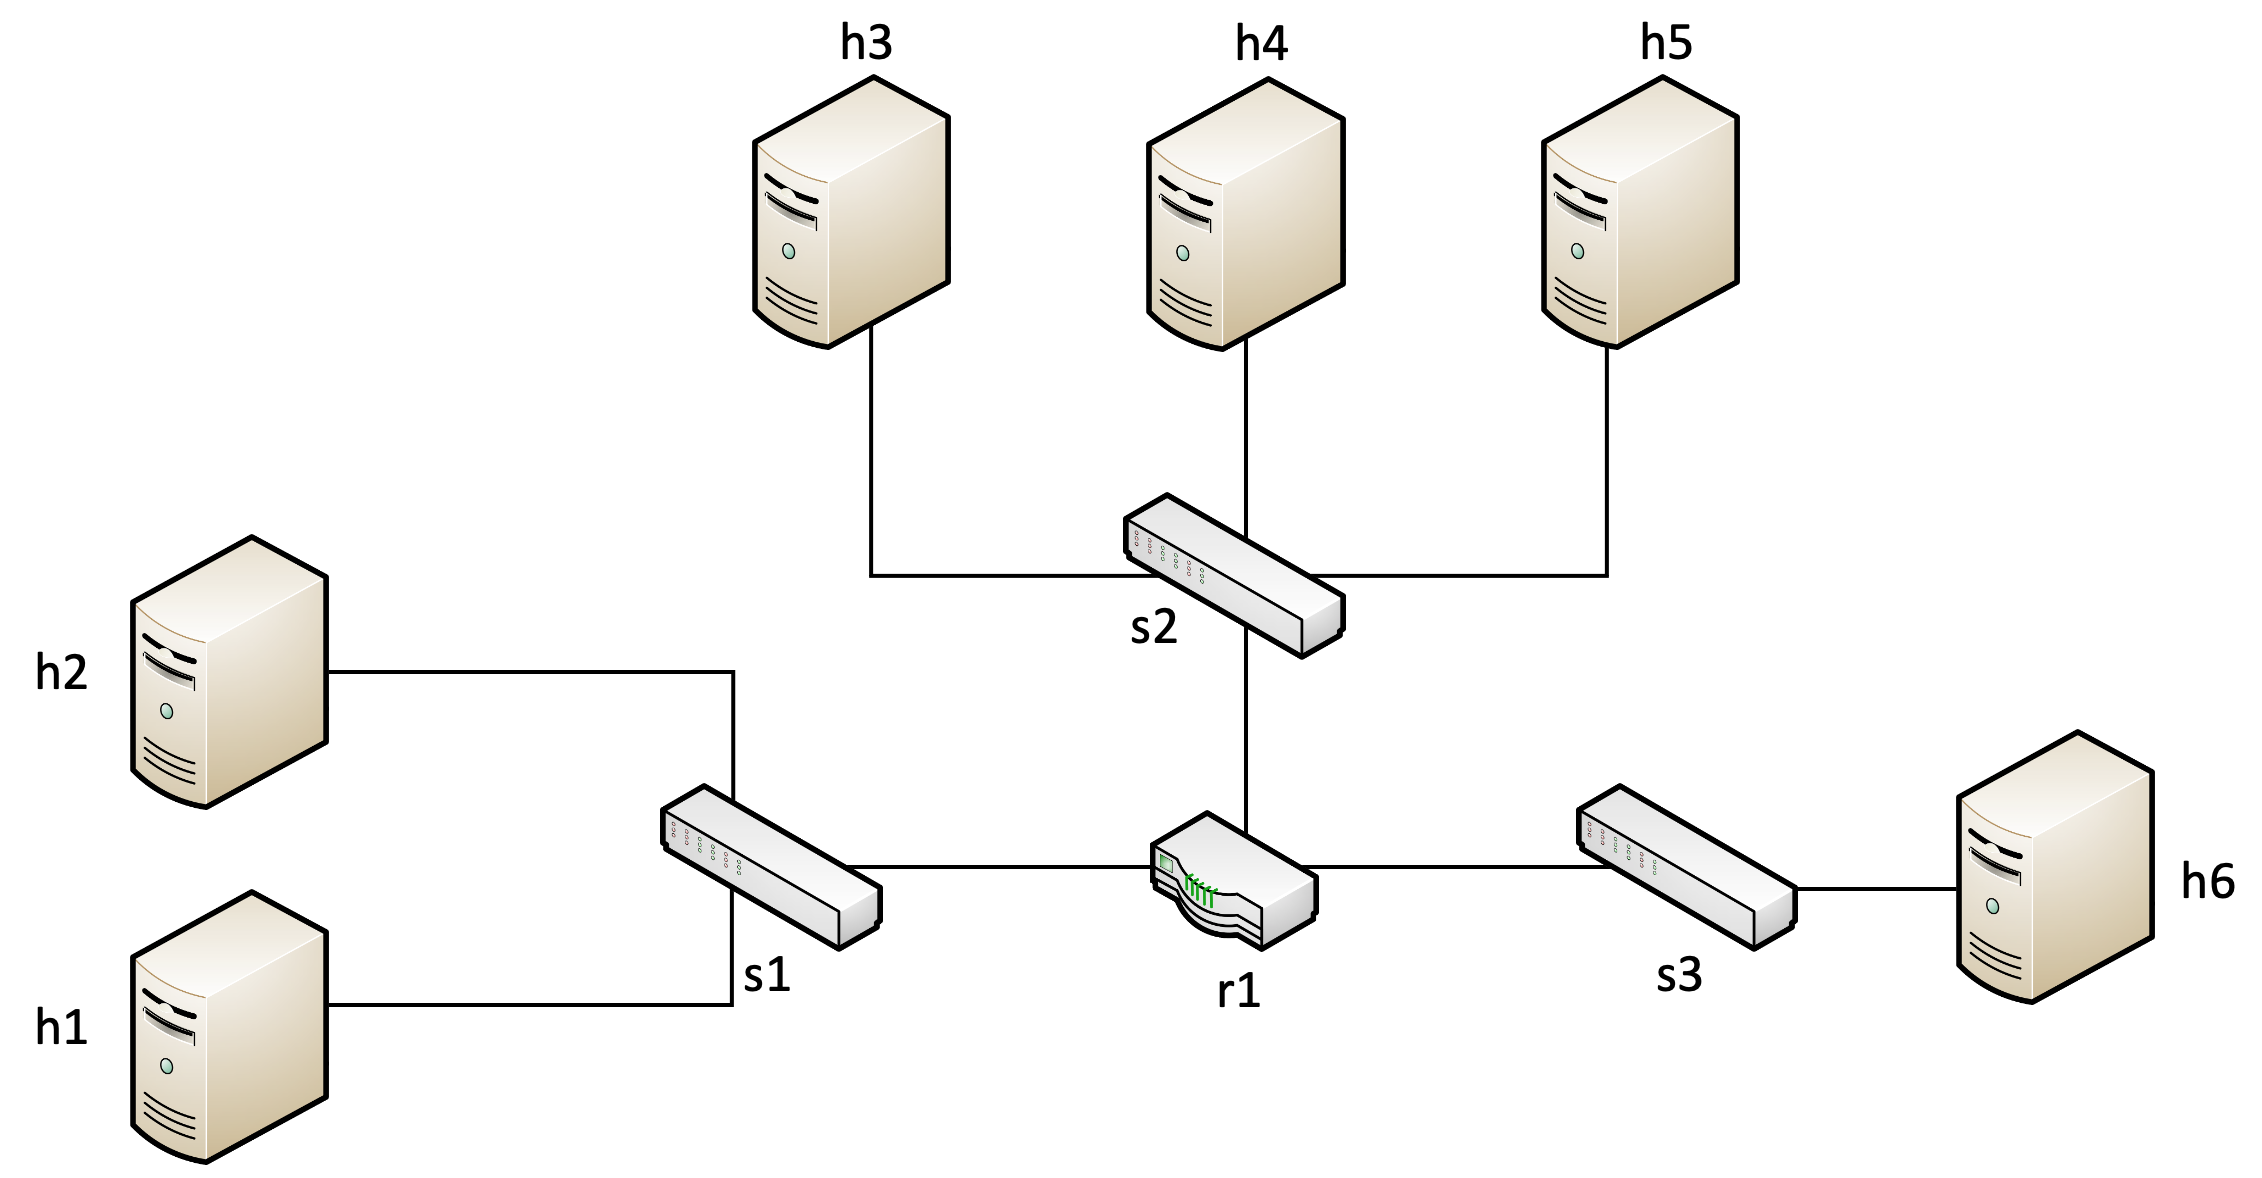
\includegraphics[width=0.8\linewidth]{graphics/Lab0-Mininet2.png}	
	\caption{Our second network topology, using 6 hosts, 3 switches and 1 router}
	\label{fig:mininet2}
\end{figure}

\begin{table}[ht]
	\centering
	\begin{tabular}{| c | c | c |}	
		\hline
		\textbf{Host} & \textbf{\ac{ipv6} address of eth0}  \\ \hline
		h1 & \texttt{fc00:0:0:1::1/64} \\ 
		h2 & \texttt{fc00:0:0:1::2/64} \\
		h3 & \texttt{fc00:0:0:2::1/64} \\
		h4 & \texttt{fc00:0:0:2::2/64} \\
		h5 & \texttt{fc00:0:0:2::3/64} \\
		h6 & \texttt{fc00:0:0:3::1/64} \\
		\hline
		r1 - eth0 & \texttt{fc00:0:0:1::10/64} \\ 
		r1 - eth1 & \texttt{fc00:0:0:2::10/64} \\ 
		r1 - eth2 & \texttt{fc00:0:0:3::10/64} \\ 
		\hline
	\end{tabular}
	\caption{\ac{ipv6} addresses for Exercise 5. The interfaces of the router are numbered from left to right.}
	\label{tab:lab1-ip-addresses}
\end{table}
\end{exercise}

\begin{exercise}{Capture Mininet packets using Wireshark}
Our virtual network also produces packets that we can capture using Wireshark, just as we did before. To capture the Mininet packets on a host, you have to follow the following steps:
\begin{enumerate}
\item Start your Python script
\item If you want to look at the packets on host h1, you use the command \incommand{xterm h1}. This opens a new terminal which is running exclusively on host h1.
\item From this new terminal, start Wireshark.
\end{enumerate}

When you have to select the interface to capture the packets from, you will see extra interfaces that correspond with the interfaces configured on your Mininet host (h1, in this case).

In this exercise we will run a http server on one of the hosts and get basic files from it using \ac{http}.
\begin{enumerate}
	\item Start the Mininet CLI using the network we created in the previous part.
	\item Python has a build-in http server we can use. To start a server on host \textbf{h2}, use the following command:
\begin{cmdblock}[gobble=2]
	% h2 python3 -m http.server --bind :: &
\end{cmdblock}
	\item Start Wireshark, and capture packets from the eth0 interface of host \textbf{h1}
	\item Use \texttt{wget} to download index file from server, use the following command:
\begin{cmdblock}[gobble=2]
	% h1 wget http://h2:8000
\end{cmdblock}
	\item Save the \ac{http} packets that were captured by Wireshark in \file{pcap}
\end{enumerate}

\end{exercise}



\newpage
\subsection{Basics of tcpdump}

Tcpdump allows you to capture traffic on a network and display the packet headers of the captured traffic. The \incommand{tcpdump} command can be used to identify network problems or to monitor network activities.

\begin{exercise}{Simple tcpdump exercise}\label{ex:tcpdump}
Use the \incommand{tcpdump} command to observe the network traffic that is generated by issuing \incommand{ping6} commands.
\begin{framed}
	If you use the \incommand{tee} or \incommand{tail} commands to simultaneously view and save the output from \incommand{tcpdump}, you need to use the \incommand{-l} option of \incommand{tcpdump}. For example:
	\begin{cmdblock}[gobble=2]
		% tcpdump -n -l > filename \& tail -f filename
		% tcpdump -n -l | tee filename
	\end{cmdblock}
	\emph{\remark It may be necessary to hit \incommand{Ctrl-c} to terminate the tcpdump session. In some situations, it may be best to simply redirect the output of tcpdump straight to a file (e.g., \incommand{tcpdump \textgreater filename}) and view it afterwards with the \incommand{less} command or a text editor.}
\end{framed}

\begin{enumerate}
	\item Start tcpdump on \textbf{h1} so that it monitors all packets that contain the \ac{ipv6} address of \textbf{h2}, by typing:
	\begin{cmdblock}[gobble=2]
	% h1 tcpdump -n host fc00:0:0:1::2 > tcpoutput.txt &
	\end{cmdblock}
	\item Send 2 pings from \textbf{h1} to \textbf{h2}
	\item Stop tcpdump:
	\begin{cmdblock}[gobble=2]
		% h1 killall tcpdump
		\end{cmdblock}
	\item Observe the output of tcpdump, which is captured in tcpoutput.txt. Rename this outputfile to \file{txt}.
\end{enumerate}

\question{Include the saved output in your lab report. Explain the meaning of each field in the captured data.}{1}

\end{exercise}

\begin{exercise}{Another tcpdump traffic capture}
\begin{enumerate}
	\item On \textbf{h1}, start capturing packets using the \incommand{tcpdump -i h1-eth0 -n} command. Don't forget to capture the output in a file.
	\item Issue a ping (limited to 2 pings) to the non-existing \ac{ipv6} address \texttt{fc00:1234::1}.
	\item Issue a ping to the special address \texttt{ff02::1}.
	\item Save the outputs of ping and tcpdump to \file{ping.txt}{} and \file{tcpdump.txt}{}, respectively.
\end{enumerate}
\end{exercise}

\question{Include the saved output in your lab report and interpret the results. What happens when you ping \texttt{fc00:1234::1}? Did you capture any packets? Why or why not? How many of the Linux PCs responded to the ping to \texttt{ff02::1}? Why is this?}{2}
